% The 16:9 "widescreen" aspectratio is entirely optional
\documentclass[aspectratio=169]{beamer}

\usetheme{collegegreen}
\usepackage{booktabs}
\usepackage{colortbl}
\usepackage{natbib}
\usepackage{hyperref}
\hypersetup{
  colorlinks=true,
  linkcolor=TrinityBlue,
  filecolor=TrinityBlue,
  urlcolor=pms_512,
  citecolor=pms_512,
}

\title{The \textit{College Green} Theme}
\subtitle{A Beamer theme for Trinity College Dublin}
\institute{Trinity College Dublin, the University of Dublin}
\author{Barra Roantree}
\date{\today}

\begin{document}

% -------------------------------------------------------
% Title slide — white canvas so the logo blends cleanly
% -------------------------------------------------------
{
\setbeamercolor{background canvas}{bg=white}
\begin{frame}
\titlepage
\end{frame}
}

% -------------------------------------------------------
% Outline
% -------------------------------------------------------
\begin{frame}{Outline}
\tableofcontents
\end{frame}

% -------------------------------------------------------
% Section 1 — Theme features
% -------------------------------------------------------
\section{Theme Features}

\begin{frame}{The \textbf{collegegreen} theme incorporates Trinity's corporate branding}
The theme uses the official TCD colour palette and (loosely) matches the visual identity
guidelines at \texttt{tcd.ie/identity}.

\begin{itemize}
  \item The colour scheme uses the official Trinity Blue (\texttt{pms\_300}, \#0569b9)
  \item Cool Grey is used for subtitles, sub-item bullets, and hyperlinks
  \item The footer bar carries the full institutional name and a frame counter
  \item The logo is embedded automatically on the title page
  \item All 13 named PMS colours — plus tint ramps — are available as named macros
  \begin{itemize}
    \item e.g.\ \texttt{\textbackslash color\{pms\_312\}} or \texttt{\textbackslash color\{pms\_280\_50\}}
  \end{itemize}
  \item The theme works well with pdf\LaTeX\ and Xe\LaTeX
\end{itemize}
\end{frame}

% -------------------------------------------------------
% Section 2 — The Long Room Library
% -------------------------------------------------------
\section{The Long Room Library}

\begin{frame}{The Long Room Library, Trinity College Dublin}
\begin{figure}
  \centering
  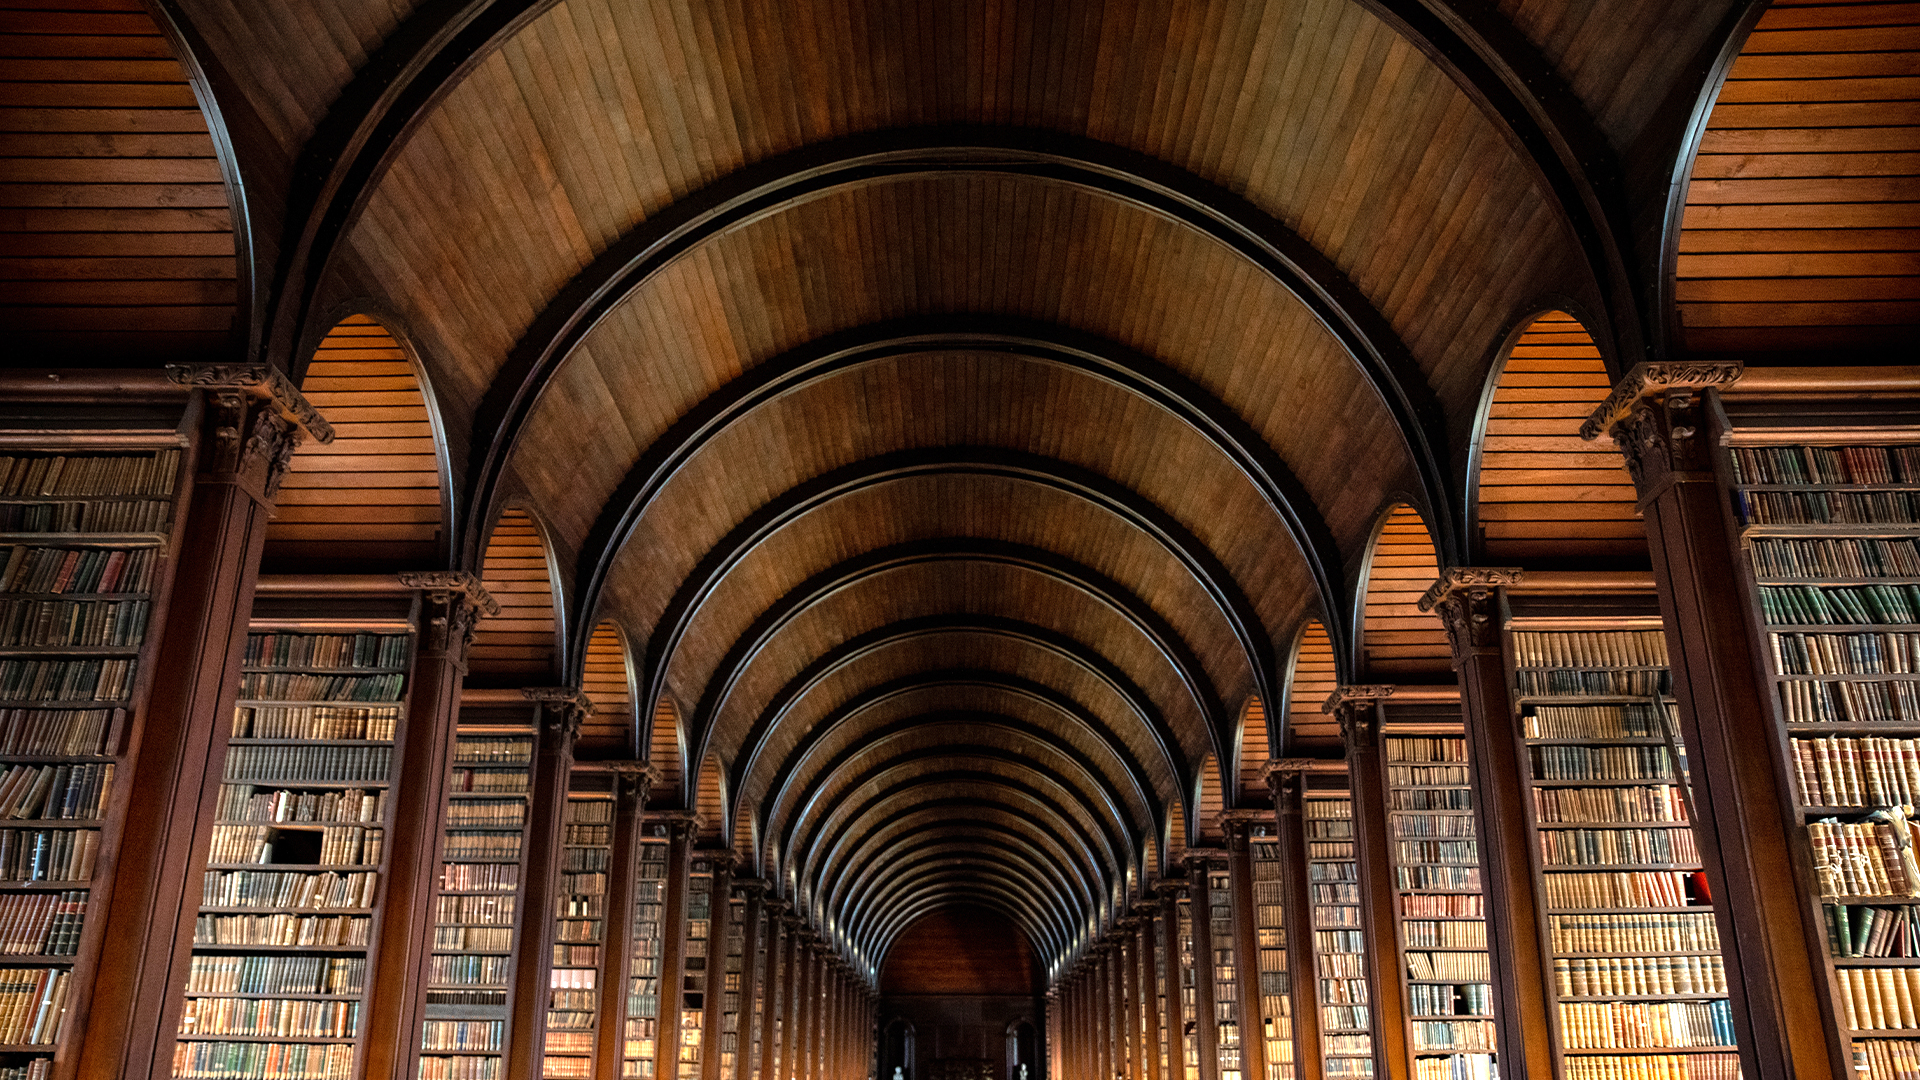
\includegraphics[width=0.82\textwidth]{trinity-virtual-background-11}
  \caption{The Long Room Library. Image \href{https://www.tcd.ie/identity/templates/virtual-backgrounds/}{available here}.}
\end{figure}
\end{frame}

% -------------------------------------------------------
% Section 3 — Colour Palette
% -------------------------------------------------------
\section{TCD Colour Palette}

\begin{frame}{TCD PMS colour palette}
\small
\renewcommand{\arraystretch}{1.3}
\begin{columns}[t]
  \begin{column}{0.48\textwidth}
    \begin{tabular}{ll}
      \toprule
      \textbf{Shorthand} & \textbf{Swatch} \\
      \midrule
      \texttt{pms\_300}      & \cellcolor{pms_300}\hspace{2cm} \\
      \texttt{pms\_coolgrey} & \cellcolor{pms_coolgrey}\hspace{2cm} \\
      \texttt{pms\_black}    & \cellcolor{pms_black}\hspace{2cm} \\
      \texttt{pms\_white}    & \cellcolor{pms_white}\hspace{2cm} \\
      \texttt{pms\_312}      & \cellcolor{pms_312}\hspace{2cm} \\
      \texttt{pms\_326}      & \cellcolor{pms_326}\hspace{2cm} \\
      \texttt{pms\_360}      & \cellcolor{pms_360}\hspace{2cm} \\
      \texttt{pms\_375}      & \cellcolor{pms_375}\hspace{2cm} \\
      \bottomrule
    \end{tabular}
  \end{column}
  \begin{column}{0.48\textwidth}
    \begin{tabular}{ll}
      \toprule
      \textbf{Shorthand} & \textbf{Swatch} \\
      \midrule
      \texttt{pms\_389}      & \cellcolor{pms_389}\hspace{2cm} \\
      \texttt{pms\_109}      & \cellcolor{pms_109}\hspace{2cm} \\
      \texttt{pms\_466}      & \cellcolor{pms_466}\hspace{2cm} \\
      \texttt{pms\_165}      & \cellcolor{pms_165}\hspace{2cm} \\
      \texttt{pms\_485}      & \cellcolor{pms_485}\hspace{2cm} \\
      \texttt{pms\_512}      & \cellcolor{pms_512}\hspace{2cm} \\
      \texttt{pms\_280}      & \cellcolor{pms_280}\hspace{2cm} \\
      \texttt{pms\_gold}     & \cellcolor{pms_gold}\hspace{2cm} \\
      \texttt{pms\_silver}   & \cellcolor{pms_silver}\hspace{2cm} \\
      \bottomrule
    \end{tabular}
  \end{column}
\end{columns}
\end{frame}

% -------------------------------------------------------
% Section 4 — References
% -------------------------------------------------------
\section{References}

\begin{frame}{In-text citations}
Citations use the author-year style. For example:

\begin{itemize}
  \item A seminal study on minimum wages used a natural experiment
        comparing New Jersey and Pennsylvania \citep{card1994}.
  \item \citet{angrist1991} estimate returns to schooling using compulsory attendance
        laws as an instrument.
  \item For a comprehensive treatment of IV and DiD methods, see \citet{angrist2009}
        or \citet{wooldridge2010}.
\end{itemize}

\vspace{\baselineskip}
{\small Click any citation to jump to the reference list.}
\end{frame}

\begin{frame}[allowframebreaks]{References}
\bibliographystyle{apalike}
\bibliography{refs}
\end{frame}

% -------------------------------------------------------
% Standout slide
% -------------------------------------------------------
\begin{frame}[standout]
Questions?
\end{frame}

\end{document}